\section{Aufbau der Visualisierung}
\begin{figure}[!htbp]
 \centering
 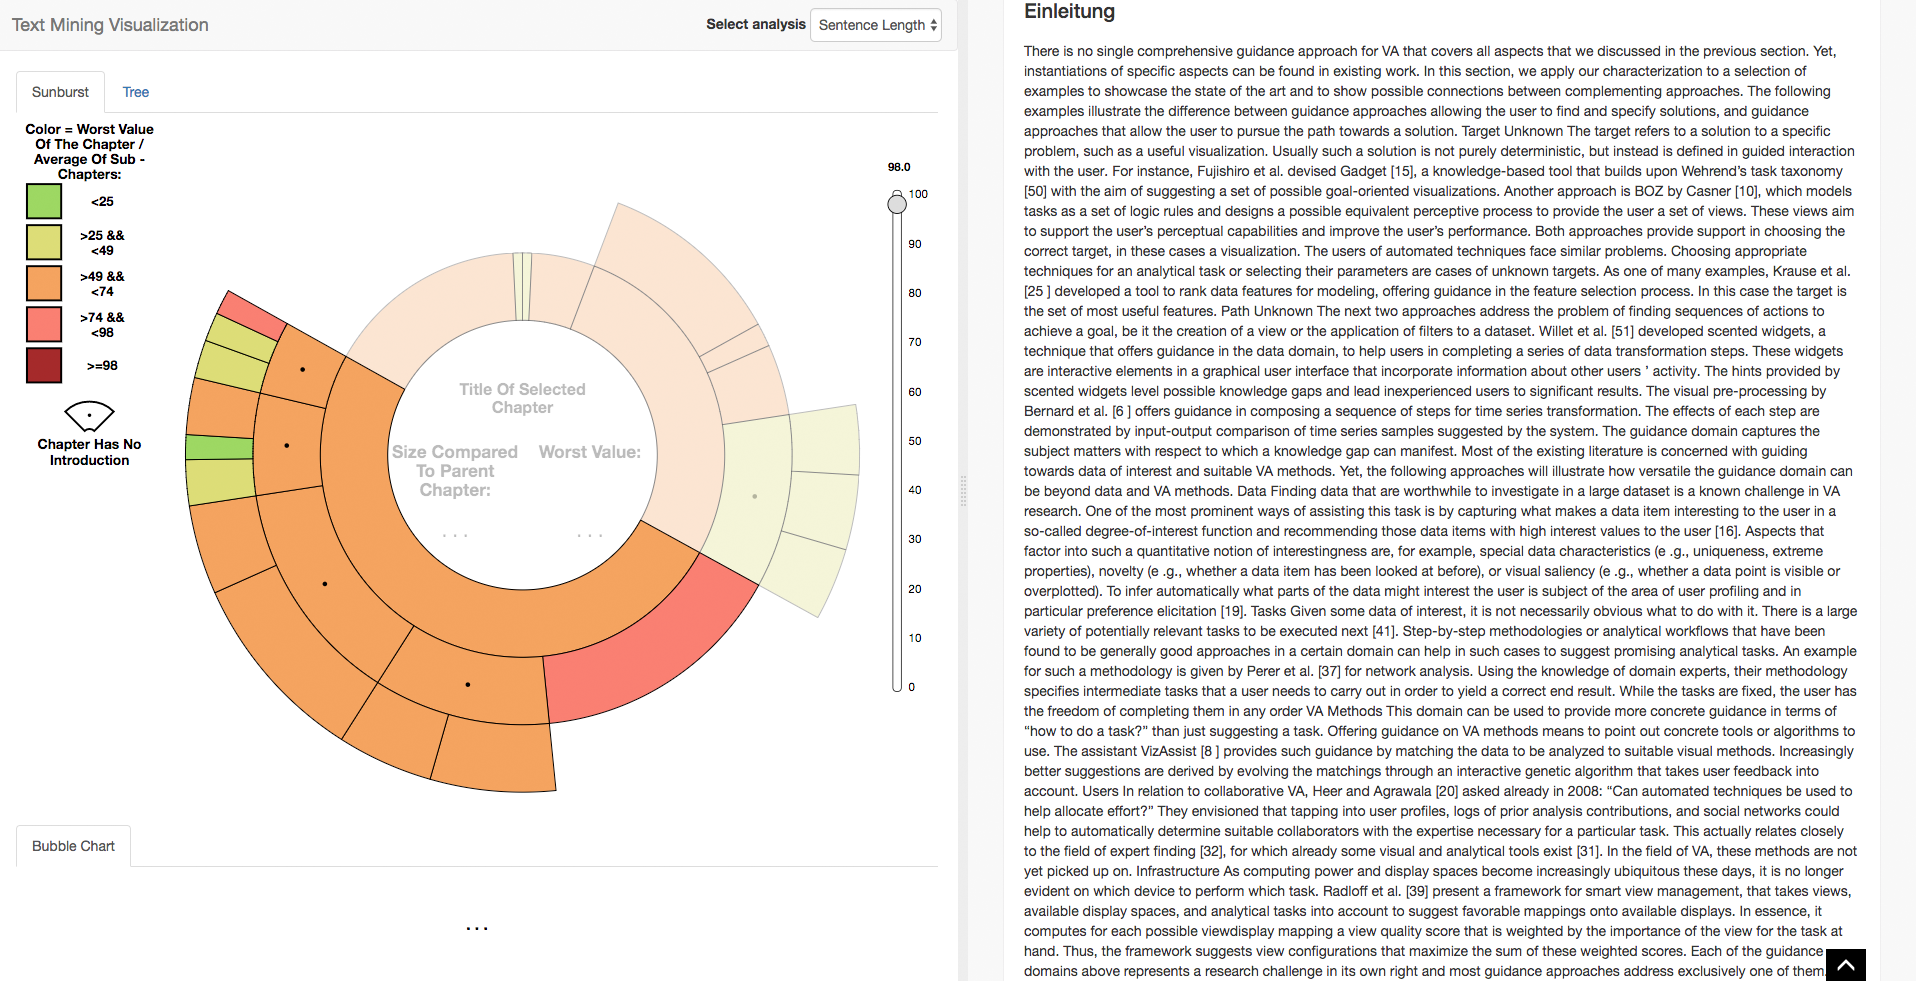
\includegraphics[width=\columnwidth]{overview}
 \caption{Startansicht der Visualisierung (links: Sunburst-Diagramm als Navigation, rechts: Betrachtetes Dokument im Text-Viewer-Fenster)}
 \label{fig:sunburst}
\end{figure}
Die Visualisierung ist in zwei Abschnitte eingeteilt, welche vertikal voneinander Abgetrennt sind und in einer starken Synergie stehen. Die Linke Seite des Bildschirms wird von der eigentlichen Visualisierung eingenommen und die rechte Seite stellt einen Text-View dar. In der Visualisierung k\"onnen verschiedenen Auswahlen getroffen und hierdurch innerhalb des Text-Views markiert werden. Anhand der textuellen Darstellung und N\"ahe der markierten Begriffe kann der Nutzer nun R\"uckschl\"usse bez\"uglich der Wissenschaftlichkeit seines Dokuments bilden und gegebenenfalls Verbesserungen an diesem vornehmen. Die Abschnitte sind durch einen Balken klar abgetrennt, welcher jedoch, jeh nach Anforderung des Nutzers, verschoben werden kann, um die Gr\"o{\ss}enverh\"altnisse anzupassen. Wird gerade eine Auswahl getroffen, so kann es n\"tzlich sein die Visualisierungsseite zu vergr\"o{\ss}ern. Wurde bereits eine Auswahl getroffen so kann die Textseite verg\"o{\ss}ert werden.\\
Um eine geeignete und feingranulare Auswahl dieser Begriffe gew\"ahrleisten zu k\"onnen, ist auch der Visualisierungsbereich in weitere, aufeinander aufbauende, Einzelvisualisierungen gegliedert. Somit beinhaltet sie:
\begin{center} 
   \begin{varwidth}{2in} 
      \begin{itemize} 
         \item eine Navigation,
		 \item eine Kapitel\"ubersicht / -auswahl,
		 \item und eine Detailansicht der Selektion. 
      \end{itemize} 
   \end{varwidth} 
\end{center} 
Jede dieser Visualisierung hat ein festes Seitenverh\"altnis, sodass eine Verzerrung durch Gr\"o{\ss}en\"anderungen vermieden wird.\\
\\
Innerhalb der Navigation wird dem Nutzer ein Drop-Down-Men\"u geboten, \"uber welches sich die Filterungsmethode definieren l\"asst (Redundanzen, Satzzeichen, Satzl\"ange oder F\"ullw\"orter). Wurde hier eine Auswahl getroffen, so wird die gesamte Visualisierung auf diese abgestimmt sodass dem Nutzer eine gezieltere Suche erm\"oglicht wird.\\
\\
Der zweite Abschnitt veranschaulicht die Hierarchie des ausgew\"ahlten Dokuments und wird f\"ur die Auswahl zu betrachtender Kapitel genutzt. Hier werden zwei alternative Ansichten geboten, eine in Form eines Sunburst und eine als Baumstruktur, welche teilweise unterschiedliche Auspr\"agungen hervorheben und sich somit gegenseitig erg\"anzen. \"Uber Tabs kann der Nutzer zu jedem Zeitpunkt die f\"ur ihn n\"utzlichere Ansicht selektieren. Wichtig ist hierbei, dass die, in den Ansichten get\"atigten, Auswahlen synchronisiert werden, wodurch ein flie{\ss}ender Wechsel unterst\"utzt wird. \\
\\
Wurde in der Kapitel\"ubersicht eine Auswahl getroffen, so wird diese in einer Detailansicht aufgegriffen. Hier sind die Begriffe der Ausgew\"ahlten Kapitel anhand der Filterungsmethode eingegrenzt und in Form eines Blasen-Diagramms visualisiert. Wurden beispielsweise Redundanzen selektiert, so steht jede Blase f\"ur ein Wort, welches innerhalb der Kapitelauswahl redundant auftritt. Zu jedem dieser Begriffe wird auch die entsprechende Auspr\"agung der Filterungsmethode bereitgestellt, sodass eine pers\"ohnliche Problemeinsch\"atzung des Nutzers erfolgen kann. Ist nun eine \"Uberarbeitung bestimmter Begriffe gew\"unscht, so k\"onnen diese selektiert und hierdurch jedes Vorkommnis, begrenzt durch die ausgew\"ahlten Kapitel, in dem Text-View markiert werden.\\
\\
Das folgende Kapitel dient somit zun\"achst der Erl\"auterung dieser Einzelvisualisierungen. Hierbei werden besonders die Entscheidungsfindungen und Kompromisse beleuchtet, welche zu dem Aufbau und den Interaktionsm\"oglichkeiten der jeweiligen Visualisierung f\"uhrten.
\newpage
\subsection{Kapitel\"ubersicht: Sunburst-Diagramm} \label{subsec:sunburst}
\begin{figure}[!htbp]
 \centering
 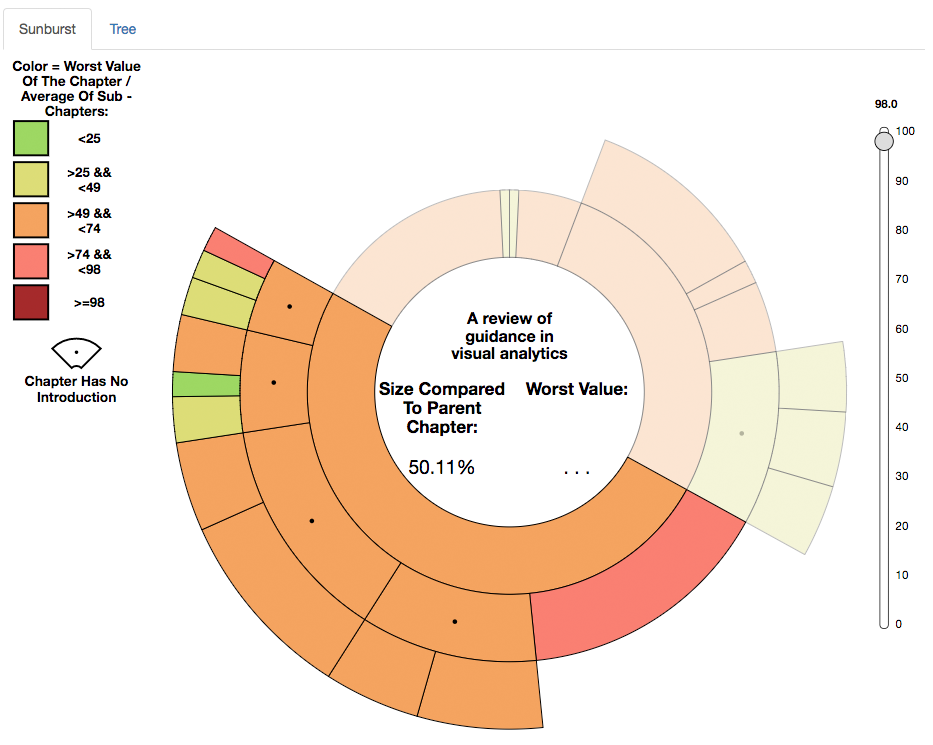
\includegraphics[width=\columnwidth]{sunburst}
 \caption{Sunburst-Diagramm als Kapitelauswahl mit Farblegende und Spezifizierungs-Slider (der Mauszeiger befindet sich \"uber dem Kapitel "A review of guidance in visual analytics")}
 \label{fig:overview}
\end{figure}

Dem Sunburst-Diagramm liegt der Gedanke zugrunde, dass der Nutzer den Aufbau des Dokuments bereits kennt, sich also im Vorhinein damit auseinander gesetzt hat und nun mithilfe der Visualisierung eine weitere Iteration vornehmen m\"ochte. Im Fokus steht hierbei die bereits gut bekannte Kapitelhierarchie zentriert und auf einen Blick sichtbar darzustellen und somit eine schnelle Navigation und Auswahl zu erm\"oglichen. Da bei solch einem Diagramm nahezu keine Freifl\"achen zwischen den Elementen gegeben sind, kann den Elementen selber weitaus mehr Fl\"ache zugeordnet werden ohne die \"Ubersichtlichkeit der Visualisierung zu gef\"ahrden. Dies f\"uhrt zu einer Maximierung der Datendichte. Die verf\"ugbare Visualisierungsfl\"ache wird also bestm\"oglich ausgenutzt, da Lediglich das Zentrum und die Ecken des Diagramms Freifl\"achen bilden, welche jedoch f\"ur Informationstexte nutzbar sind. Bei einer Verkleinerung des Diagramms sind einzelne Abschnitte somit trotzdem klar erkenn- und trennbar, sodass die Visualisierung problemlos auf unterschiedlichen Bildschirmgr\"o{\ss}en angezeigt und genutzt werden kann.\\
\\
Ein weiterer Beweggrund f\"ur diese Art der Darstellung war, dass dem Nutzer ein Auswahlmedium bereitgestellt werden soll, welches die Dokumenthierarchie sowie Kapitel-Abh\"angigkeiten veranschaulicht. Durch die Aufeinanderschichtung der unterschiedlichen Ringlagen dieser Diagrammart sind die genannten Abh\"angigkeiten schnell erkennbar. Es werden keine weiteren visuellen Mittel ben\"otigt um die Zugeh\"origkeit eines Kapitels zu verdeutlichen, da die Position der Elemente ausreichend Aufschluss hier\"uber bietet. Somit wird auch die Data-Ink-Ratio erh\"oht und Chartjunk vermieden. Der mittlere Kreis stellt hierbei das Dokument dar, welches zun\"achst von den Hauptkapiteln (Abstract, Einleitung, Hauptteil, Fazit, etc.) umringt wird. Die Gr\"o{\ss}e des jeweiligen Ringabschnitts, in Abh\"angigkeit des Radius, ist hierbei der prozentuelle Anteil des Kapitels im Verh\"altnis zum gesamten Dokument. Als Ma{\ss} gilt hier die Wortanzahl eines Kapitels, welche sich aus dem eigenen Inhalt, sowie dem Inhalt aller Unterkapitel erschlie{\ss}en l\"asst und anschlie{\ss}end auf den entsprechenden Teilwinkel des Kreises umgerechnet wird. Dieses Schemata erstreckt sich auch auf die Unterkapitel eines Abschnittes, welche jedoch nun ihr jeweiliges Elternkapitel als Maximum ansehen (sowohl deren radialen Abschnitt in der Visualisierung als auch deren Wortanzahl) und nicht das gesamte Dokument.\\
\\
Ein Vorteil der hierdurch entsteht ist, dass neben der sichtbaren Hierarchie auch ein Gr\"o{\ss}enverh\"altnis zum jeweiligen Oberkapitel ersichtlich wird. F\"ur wissenschaftliche Arbeiten bestehen h\"aufig formale Anforderungen, sodass auch die Gr\"o{\ss}e einzelner Kapitel vorgegeben sein kann. Somit k\"onnte es also n\"utzlich sein solche Verh\"altnisse aus der Visualisierung entnehmen zu k\"onnen. Hierbei wurde jedoch bedacht, dass Gr\"{\ss}enverh\"altnisse in Kreisdiagrammen tr\"ugen k\"onnen, da der radiale Abschnitt die Gr\"o{\ss}e eines Ringabschnitts definiert und somit \"au{\ss}ere Abschnitte aufgrund ihrer Fl\"ache automatisch gr\"o{\ss}er erscheinen als Innere (auch bekannt als Lie Factor oder L\"ugenfaktor). Da bei der \"Uberarbeitung eines wissenschaftlichen Textes jedoch vorwiegend das direkte Verh\"altniss eines Kapitels zu Nachbarkapiteln des selben Oberkapitels betrachtet wird, wurde dieser Aspekt im Kontext des Projektes als vernachl\"assigbar eingesch\"atzt. Im Sunburst-Diagramm besitzen zudem alle Lagen die selbe H\"ohe, sodass der Fl\"acheninhalt hier eine geringere Bedeutung als der dargestellte Radius besitzt und somit trotzdem eine akkurate visuelle Einsch\"atzung get\"atigt werden kann. Damit der eigene Textanteil eines Oberkapitels ebenfalls mit den Textanteilen der Unterkapitel verglichen werden kann, wurde entschieden auch diesen Anteil als Unterkapitel aufzulisten und ihn somit auf deren Ebene zu verschieben. Diese werden jedoch als Einleitung betitelt und somit durch ihre Namensgebung speziell gekennzeichnet, sodass die Zugeh\"origkeit bestehen bleibt. Dies ist jedoch nur ben\"otigt, wenn ein Kapitel weitere Kapitel umschlie{\ss}t. Ansonsten wird der Textinhalt weiterhin im eigenen Element dargestellt.\\
\\
Da in einem wissenschaftlichen Dokument jedes Kapitel eine Einleitung besitzen sollte und dieses nicht direkt aus der bisherigen Visualisierung hervorgeht, wurde zudem eine M\"oglichkeit gesucht, fehlenden Text aufzuzeigen. Sollte also ein Kapitel keinen eigenen Text beinhalten, so wird in der Mitte des zugeh\"horigen Elements ein schwarzer Kreis gezeichnet. Dieser nimmt wenig Platz ein, wodurch die Data-Ink-Ratio nahezu unbeschadet bleibt. Durch die nun entstandene Unregelm\"a{\ss}igkeit innerhalb der Visualierung ist er jedoch auf den ersten Blick klar erkennbar, sodass dem Nutzer das Problem direkt \"ubermittelt wird.\\
\\
Ein weiterer wichtiger Aspekt dieser Visualisierung findet sich in der Farbgebung der Abschnitte. Da die Farbe ein gutes visuelles Mittel zur \"Ubermittlung der Qualit\"at eines Elements ist, wird sie hier zu exakt jenem Zweck verwendet. Anhand der ausgew\"ahlten Filterungsmethode werden die jeweiligen Auspr\"agungen der Kapitel berechnet und diese anschlie{\ss}end in dem zugeh\"origen Farbton dargestellt. Bei der Auswahl der Farbe gilt der h\"ochste ermittelte Wert innerhalb eines Kapitels als ma{\ss}gebend f\"ur diese Einf\"arbung. Dies ist damit begr\"undet, dass besonders Ausrei{\ss}er erfasst und sichtbar gemacht werden sollten, welche bei der Bildung eines Durchschnitts verborgen bleiben k\"onnten. Wurde beispielsweise die Filterungsmethode bez\"uglich der Satzl\"ange ausgew\"ahlt, so k\"onnte bei der Durchschnittsbildung ein sehr langer Satz \"ubersehen werden, welcher jedoch die Qualit\"at des Dokumentes beeintr\"achtigt. Diese Einf\"arbung wird f\"ur jedes Kapitel eigenst\"andig vorgenommen. Dies ist damit begr\"undet, dass es Worth\"aufigkeiten gibt, welche einen hohen Einfluss auf die Textqualit\"at eines Unterkapitels haben, jedoch verglichen mit dem Oberkapitel unauff\"allig erscheinen. Ebenso k\"onnte in einem Oberkapitel eine Worth\"aufigkeit als problematisch angesehen werden, diese jedoch gleichm\"a{\ss}ig auf die Unterkapitel aufgeteilt sein und somit f\"ur diese nur eine geringe Auswirkung haben. Diese Aspekte sind nun direkt aus der Visualisierung entnehmbar, sodass die Trennung dem Nutzer eine gezieltere und schnellere Suche erm\"oglicht.\\
\\
Bei der Farbwahl wurde von einer linearen Interpolation zwischen zwei Farbt\"onen abgesehen und sich stattdessen f\"ur eine klar unterteilte Skala mit den Farbt\"onen Gr\"un, Gelb, Orange, Hellrot und Dunkelrot entschieden. Die Farbt\"one wurden so gew\"ahlt, da die Endt\"one im Kompliment\"arkontrast stehen, also eine einfache Unterscheidung der Qualit\"at stattfinden kann. Zudem soll dem Nutzer \"uber diese Farbgebung eine direkte Assoziation mit der gew\"unschten Aussage erm\"oglicht werden, da ein Gr\"unton allgemein positives Feedback symbolisiert und ein Rotton vorwiegend als Gefahrensignal aufgefasst wird (Ampelprinzip). Auch wenn die letzten beiden Farbt\"one den Grundton Rot besitzen, sind sie dennoch durch ihre S\"attigung klar trennbar, sodass eine Qualit\"atsminderung erkenntlich wird. Weiterhin wurde die Skala auf f\"unf Untert\"one reduziert. Auch hier ist wieder ein Argument, dass die T\"one klar trennbar sein sollten und dies bei einer gr\"o{\ss}eren Anzahl von Unterfarben nicht mehr gegeben w\"are. Weiterhin ist es Ziel dieser Visualisierung dem Nutzer eine klare Einteilung der Qualit\"at zu bieten, ebenso wie eine kurze Eingew\"ohnungsphase. Eine h\"ohere Anzahl der Unterteilungen k\"onnte die Eingew\"ohnungszeit verl\"angern.\\
Nun kann es vorkommen, dass unterschiedliche Nutzer auch unterschiedliche Anforderungen an ihr Dokument stellen. Ist die Zeit knapp, so steht beispielsweise die schnelle Identifikation der schwerwiegendsten Probleme im Vordergrund. Hat der Nutzer mehr Zeit oder sind strengere Regelungen an das Dokument gekettet, so sollten auch geringere Problemstellen aufgezeigt und beseitigt werden. Aus diesem Grund wurde den Farben kein fester numerischer Wert zugeordnet. F\"ur die Zuordnung dieser Werte wurde ein Slider integriert, mit welchem der Nutzer definieren kann, ab welcher Auspr\"agung ein Kapitel dunkelrot eingef\"arbt wird. Diese Obergrenze wird nun zudem in vier gleichm\"a{\ss}ig verteilte Unterbereiche aufgeteilt und den einzelnen Farbwerten zugeordnet. Durch die Anpassung der Einf\"arbung und die Gr\"o{\ss}e der Kapitel kann der Nutzer nun eine geeignete Strategie bzw. Reihenfolge der Textbearbeitung festlegen. Wurde beispielsweise der Wert zehn als Obergrenze definiert, so zeigen sich folgende Zuordnungen:\\
\begin{center} 
   \begin{varwidth}{2in} 
      \begin{itemize} 
         \item[Gr\"un:] Werte von 0 bis 2,5 
		 \item[Gelb:] Werte von 2,5 bis 5
		 \item[Orange:] Werte von 5 bis 7,5
		 \item[Hellrot:] Werte von 7,5 bis 10
		 \item[Dunkelrot:] Werte ab 10
      \end{itemize} 
   \end{varwidth} 
\end{center} 
Innerhalb einer Recherche wurden leider keine Richtwerte f\"ur die einzelnen Kategorien gefunden, sodass vorerst Beispielwerte anhand der vorliegenden Datenstrukturen definiert wurden. In weiteren Schritten sollten hier durch Studien genauere Richtlinien ermittelt und die bisherigen Skalen angepasst werden.\\
\\
Ver\"andert sich jedoch der Kontext durch die Auswahl einer anderen Filterungsmethode, so werden auch andere Auspr\"agungen betrachtet. Tritt ein Wort redundant auf, sollte dessen Anzahl im Verh\"altnis zum jeweiligen Paragraphen betrachtet werden. Wird hingegen nach der Satzl\"ange oder der Anzahl von Satzzeichen gesucht, so ist eine Angabe der maximalen Wort- oder Satzzeichenanzahl eines kritischen Satzes sinnvoller. Da die Werte des Sliders somit nicht auf jede Filterungsmethode gleichzeitig abgestimmt werden kann, wurden jeweils Obergrenzen und Inkrementierungsschritte in Form von unterschiedlichen Skalen definiert. Durch diese Vorauswahl wird der Slider nun auf den jeweiligen Kontext angepasst, jedoch weiterhin eine starke Anpassung des Nutzers erm\"oglicht.\\
\\
Damit dem Nutzer stets bekannt ist, welcher Farbe welcher Wertebereich zugeordnet ist, sind diese Zusammenh\"ange auf der linken Seite in Form einer Legende aufgelistet. Wird der Slider bewegt und losgelassen, so werden die neuen Unterabschnitte direkt berechnet und innerhalb der Legende angepasst. Neben der Farbgebung werden in dieser Legende zudem ungew\"ohnliche Aspekte dieser Visualisierung aufgegriffen. So findet sich hier beispielsweise eine kurze erkl\"arung der Punkte, welche fehlenden Text darstellen.\\
\\
Weitere wichtiger Aspekt jeder Visualisierung sind dessen Interaktionsm\"oglichkeiten. Eine dieser Interaktionen bildet in dieser Visualisierung das Hervorheben eines Kapitels sobald der Mauszeiger das zugeh\"orige Element betritt. Standardm\"a{\ss}ig besitzen die Kapitelelemente eine niedrige S\"attigung, welche nun erh\"oht wird und somit ein klare Trennung von selektierten und nicht selektierten Kapiteln bewirken soll. Hierdurch wird dem Nutzer eine direkte R\"uckmeldung und dadurch ein Auffordrungscharakter geboten, welcher den Nutzer zu weiteren Interaktionen und Erkundungen animieren soll. Um diesen Effekt zu verst\"arken wurde an den einzelnen Objekten ein schmaler schwarzer Rahmen angebracht. Auch wenn dieser wiederum Chartjunk darstellt, welcher in dieser Visualisierung weitestgehend umgangen wurde, so sorgt er durch die dunklen Abgrenzungen f\"ur eine st\"arkere Hevorhebung der Auswahl und wurde somit als sinnvoll erachtet. 
Durch den Mouse-Over werden zus\"atzlich die Texte im Zentrum des Sunburst-Diagramms angepasst, welche nun den Titel des Ausgew\"ahlten Kapitels, sowie dessen h\"ochste Auspr\"agung im Bezug auf die Filterungsmethode und den prozentualen Anteil zum Oberkapitel anzeigen. Ist der Titel zu lang f\"ur den inneren Bereich des Diagramms, so wird er abgek\"urzt, dieses jedoch durch die beif\"ugung dreier Punkte gekennzeichnet. Da dem Nutzer jedoch die Struktur bekannt ist, sollte dieser Ausschnitt f\"ur eine Zuordnung ausreichend sein. Somit erh\"alt der Nutzer stets ausreichend Auskunft \"uber dieses Kapitel, welche die angesprochenen optischen Verh\"altnisse komplettieren. Besitzt das ausgew\"ahlte Kapitel Unterkapitel, so werden auch diese Hervorgehoben und die Gesamtgr\"o{\ss}e dieser als Grundlage f\"ur die Informationstexte genommen. Auf diese Weise kann eine m\"oglichst flexible Erkundung des Dokuments gew\"ahrleistet werden. Verl\"asst der Mauszeiger das Kapitel, so wird auch die Auswahl r\"uckg\"angig gemacht.\\
Hat sich der Nutzer jedoch entschieden ein Kapitel genauer zu betrachten, so kann er es, zusammen allen Unterkapiteln, \"uber einen Linksklick an seine Auswahl binden und den restlichen Visualisierungen zur Verf\"ugung stellen. Verl\"asst der Mauszeiger nun das Kapitel, so wird dieses nicht mehr Abgew\"ahlt. Ist ein Element bereits ausgew\"ahlt, so wird dieses durch einen weiteren Klick aus der Auswahl entfernt. Auf diese Weise k\"onnen nahe gelegene Abschnitte parallel in den anderen Visualisierungen analysiert werden.\\
Eine parallele Auswahl mehrerer Hauptkapitel wird hierbei jedoch nicht unterst\"utzt. Dies liegt zun\"achst an der Form der Datenstruktur. Solch eine Auswahl h\"atte den Nachteil, dass eine Menge Vorberechnungen auf Seiten des Front-Ends durchgef\"uhrt werden m\"ussten, was zu ungewollten Ladezeiten f\"uhren k\"onnte. Weiterhin ist eine Einzelselektion sinnvoll, da Unterkapitel meist das selbe Thema aufgreifen und beleuchten. Hierbei besteht eine hohe Wahrscheinlichkeit f\"ur ungewollte Wiederholungen, welche es nun in dem ganzen Abschnitt zu beseitigen gilt. Wird jedoch ein Unterkapitel eines anderen Oberkapitels ausgew\"ahlt, so ist dieser Zusammenhang oft nicht gegeben. Um Verf\"alschungen oder Verdeckungen von Problemstellen entgegenzuwirken, wird in diesem Falle die vorherige Auswahl verworfen und der angeklickte Abschnitt als neue Auswahl gespeichert. Findet der Klick au{\ss}erhalb oder im Zentrum des Diagramms statt, so wird die gesamte Auswahl zur\"uckgesetzt. Hierdurch werden dem Nutzer alle M\"oglichkeiten geboten, welche er f\"ur eine erste grobe Einsch\"atzung und Auswahl der Kapitel ben\"otigt.\\
M\"ochte der Nutzer nun ein weiters Unterkapitel des gleichen Hauptkapitels (dargestellt durch die innerste Ringschicht) \"uber einen Klick an die Auswahl binden, so wird dieses der bereits get\"atigten Sammlung beigef\"ugt
\\
Eine letzte Interaktion betrifft die eigentliche Navigation durch das Textdokument. Wird ein Kapitel innerhalb des Diagramms angeklickt, so wird auch der Text-Viewer auf die Auswahl abgestimmt. Da sich das Sunburst-Diagramm auch bei geringer Gr\"o{\ss}e nutzen l\"asst, kann es zudem  als eine Art Inhaltsverzeichnis fungieren, \"uber welches nun das Dokument erkundbar ist. In jedem Falle kann die Kapitel\"ubersicht und somit auch dieses Sunburst-Diagramm als Br\"uckenst\"uck zwischen dem Textdokument und der Visualisierung gesehen werden, welches den Startpunkt jeglicher Interaktion darstellt.

\subsection{Kapitel\"ubersicht: Baum-Diagramm} \label{subsec:tree}
\begin{figure}[!htbp]
 \centering
 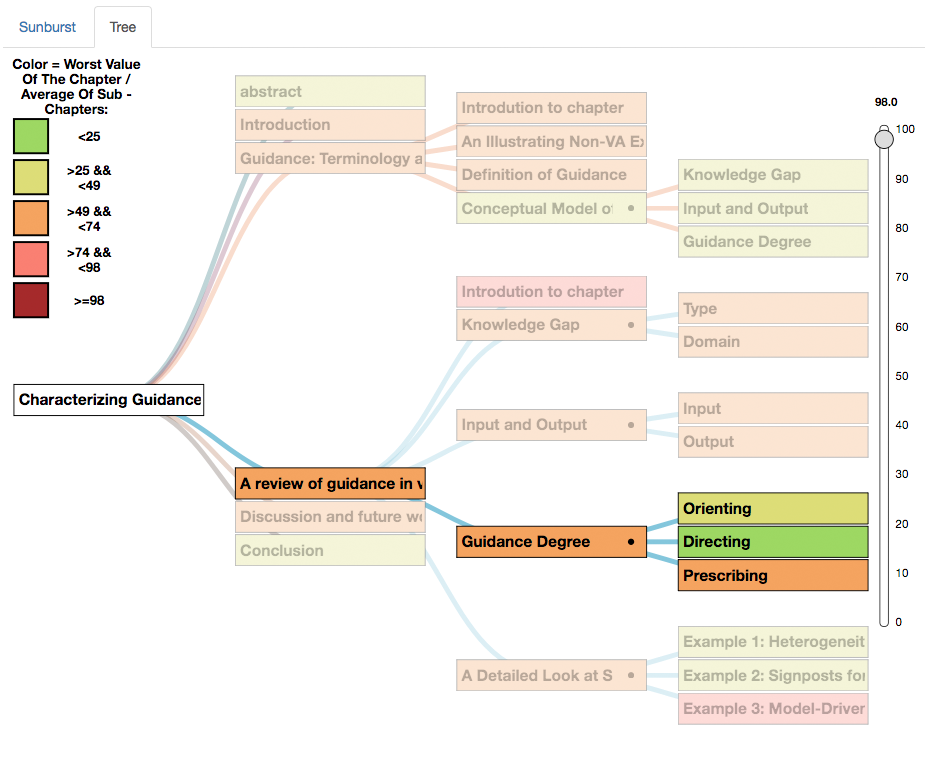
\includegraphics[width=\columnwidth]{tree}
 \caption{Baum-Diagramm als Kapitelauswahl mit Farblegende und Spezifizierungs-Slider}
 \label{fig:tree}
\end{figure}
\"Ahnlich dem Sunburst-Diagramm steht auch bei dieser Visualisierung die Darstellung der Kapitelhierarchie im Vordergrund. Dem Nutzer soll ein \"Uberblick \"uber das Dokument geboten werden, sodass eine strukturierte Bearbeitung erm\"oglicht wird. Der gr\"o{\ss}te und ma{\ss}gebliche Unterschied zur vorherigen Visualisierung findet sich jedoch in der fokussierten Zielgruppe. Das Sunburst-Diagramm ist auf jene Personen ausgelegt, welche ihr eigenes Dokument \"uberarbeiten wollen und sich somit exzellent in diesem Auskennen. Das ist der Grund, warum solch eine zentrierte Form und minimalistische Beschriftung als Ausreichend erachtet wurde. Wird sie jedoch einer Drittperson angeboten, so ben\"otigt diese eine l\"angere Einarbeitungsphase um sich zun\"achst mit den einzelnen Kapiteln vertraut zu machen. Da jedoch auch diese Personengruppe zu ber\"ucksichtigen ist, wurde an einer weiteren Visualisierung gearbeitet, welche nun Zweitpr\"ufern oder anderen Korrekturlesern dienlich ist. Hierbei wurde versucht m\"oglichst gleiche Visualisierungsmittel und Interaktionsmethoden zu verwenden, sodass ein flie{\ss}ender \"Ubergang zwischen den zwei Ansichten stattfinden kann. Hat sich ein Nutzer nun beispielsweise durch die Baumstruktur ausreichend mit den Kapiteln auseinander gesetzt, so kann dieser ohne Probleme zu der Sunburst-Ansicht wechseln. Aufgrund der weitgehenden \"Ubereinstimmungen befasst sich der folgende Abschnitt nun vorwiegend mit den Ma{\ss}gebenden \"Anderungen, welche auf diese neue Zielgruppe abgestimmt sind.\\
\\
Die Baum-Struktur wurde hier gew\"ahlt, da sie die Vernetzung der Kapitelstruktur \"ubersichtlich aufgliedert. \"Ahnlich dem Sunburst spielt auch hier die Position der Knoten eine wichtige Rolle. Diese ist optisch am einfachsten wahrzunehmen und somit der Orientierung des Nutzers sehr dienlich. Dieser Aspekt wird durch die anzeige der \"Aste unterst\"utzt. Auch wenn solche \"Aste einen hohen Anteil des Chartjunks der Visualisierung ausmachen, bieten sie in dem Kontext mehr positive als negative Aspekte. Der unwissende Nutzer findet sich schnell zurecht, da er lediglich den einzelnen Ver\"astelungen folgen muss um das gew\"unschte Kapitel zu erreichen. Hierdurch bieten sie bereits auf den ersten Blick ausreichend Orientierungspunkte, sodass Zusammen\"hange zwischen den Kapiteln schnell erkannt werden k\"onnen. Um diesen Aspekt weiterhin zu unterst\"utzen, wurden dezente, jedoch klar voneinander trennbare Farben ausgew\"ahlt. Diese sind in Form einer ordinalen Skala eingebunden, sodass sie eindeutig einem Hauptkapitel und somit dessen Ver\"astelungen zugeordnet werden k\"onnen.\\
\\
Weiterhin wurde ein horizontaler Aufbau der Baumstruktur gew\"ahlt, welcher die gewohnte Leserichtung aufgreift und dem Nutzer somit unterbewusst eine Hilfestellung bietet. Ein weiterer ma{\ss}geblicher Unterschied findet sich in der Kapitelbeschriftung. Im Sunburst wurde diese lediglich im Zentrum angebracht, da einzelne Ringe unter umst\"anden zu klein f\"ur eine ausgiebige Beschriftung sein und die Kr\"ummung den Lesefluss beeinflussen k\"onnten. Da diese Aspekte jedoch nicht auf die Knoten eines Baumes zutreffen, sind hier die Beschriftungen stets innerhalb der Knoten angebracht. Im Gegensatz zu dem stark zentrierten Aufbau des Sunburst-Diagramms ist eine Baumstruktur von Natur aus breitfl\"achiger. Da die x-Achse bei horizontalen B\"aumen deren Tiefe bestimmt und diese in einem wissenschaftlichen Dokument eine maximale Auspr\"agung von vier oder (in Ausnahmef\"allen) f\"unf besitzt, kann den einzelnen Knoten eine ausreichende Breite zur Verf\"ugung gestellt werden, wodurch auch die Titelbeschriftung profitiert. Sollte jedoch der Fall eintreten, dass ein Titel \"uber den Rand des Knotens hinaus gehen w\"urde, so wird dieser mithilfe eines Clip-Path eingeschr\"ankt. F\"ur solche F\"alle besteht die M\"oglichkeit, sich den vollst\"andigen Titel \"uber einen Hover-Effekt anzeigen zu lassen. Hierzu muss die Maus lediglich f\"ur kurze Zeit auf dem Element ruhen.\\
\\
Im Gegensatz zum Sunburst wird die Kapitelgr\"o{\ss}e in dieser Visualisierung nicht beachtet. Einer Einfindung in die Datenstruktur wird hier der h\"ochste Stellenwert zugesprochen. Die repr\"asentativste Veranschaulichung der Kapitelg\"o{\ss}en w\"are anhand der proportionalen Gr\"o{\ss}e oder Position des jeweiligen Knotens. Dies w\"urde jedoch die Kapitelhierarchie oder Anzeige der Titel beeintr\"achtigen, welche als Hauptorientierungspunkte gelten. Fehlt einem Kapitel jedoch die Einleitung oder allgemein Text, so wird dies auch hier mit einem Kreis markiert. Dieser befindet sich jedoch nicht im Zentrum des Elements, sondern an dessen Ende, sodass auch hierdurch kein Titel beeintr\"achtigt wird. \\
\\
Abgesehen von diesen Aspekten finden sich nur geringe \"Anderungen. Die Farbgebung der Knoten wird anhand der selben Aspekte ermittelt und auch der Slider zur explorativen Spezifikation der Auspr\"agungen wird beibehalten. Auch die Legende findet sich an der selben Stelle. Lediglich die Auswirkungen der Interaktion mit dem Diagramm wurden geringf\"ugig angepasst. Wird der Mauszeiger \"uber ein Element bewegt, so folgt weiterhin die Anzeige des gefilterten Wertes dieses Kapitels, da er f\"ur eine Verfeinerung der Auswahl ben\"otigt wird. Dieser ist hier jedoch an den Hover-Text des jeweiligen Elementes gebunden, welcher zudem den Titel des Kapitels Anzeigt. Das Gr\"o{ss}enverh\"altnis zum jeweiligen Oberkapitel wird hierbei jedoch nicht angebracht, da der Gr\"o{\ss}e hier im Allgemeinen zu Gunsten der Leserlichkeit weniger Beachtung geschenkt wird. Eine letzte \"Anderung findet sich in der Markierung von Kapiteln. Im Gegensatz zum Sunburst-Diagramm wird hier nicht nur das ausgew\"ahlte Element zusammen mit dessen Unterkapiteln hervorgehoben, sondern auch der Pfad vom Root-Element zu diesem Knoten sowie alle zugeh\"origen Ver\"astelungen der Auswahl. Dies ist wiederum damit begr\"undet, dass diese Visualisierung vorwiegend von dokumentfremden Personen genutzt wird und ihnen die Auswahl auf diese Weise nachvollziehbarer dargestellt wird.


\subsection{Detailansicht: Blasen-Diagramm}\label{subsec:bubble}
\begin{figure}[!htbp]
 \centering
 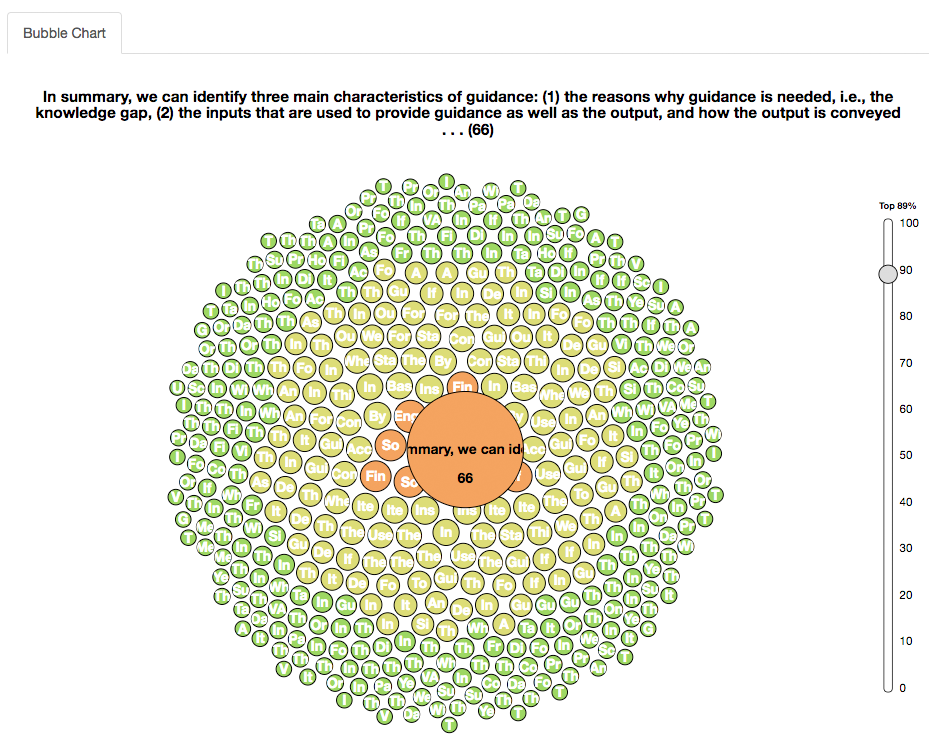
\includegraphics[width=\columnwidth]{bubble}
 \caption{Blasen-Diagramm als Detailansicht (der Mauszeiger befindet sich \"uber dem vergr\"o{\ss}erten Element)}
 \label{fig:bubble}
\end{figure}
Wurde eine Auswahl in der Kapitel\"ubersicht getroffen, werden dem Nutzer nun innerhalb der Detailansicht genauere Informationen geboten. Hier sind nun, in Abh\"angigkeit der Filterungsmethode, s\"amtliche Begriffe in Form eines Blasen-Diagramms aufgelistet. Wird nach den Redundanzen gesucht, so symbolisiert jede Blase ein Wort, welches redundant in dem ausgew\"ahlten Bereich auftritt. Wurden Satzl\"ange oder Satzzeichen selektiert, so bildet jede Blase einen Satz ab. Die Suche nach F\"ullworten hebt sich hier jedoch durch dessen Pr\"asentation etwas von den Restlichen Filterungen ab. Hierbei steht jede Blase f\"ur einen Paragraphen innerhalb der Kapitelselektion. Diese Variante wurde gew\"ahlt, da F\"ullw\"orte eine eigene Kategorie bilden, welche durch die Masse aller beinhalteter Einzelworte sch\"adlich sein kann. Mehrer F\"ullw\"orter h\"aufig verwendet worden, so ist dies ebenso schlimm, wie das Auftreten eines einzelnen F\"ullwortes in der selben Anzahl. Die Aufteilung nach Paragraphen wurde hier also gew\"ahlt, um die Suche weiterhin spezifizieren zu k\"onnen.\\
\\
Damit die einzelnen Blasen voneinander unterschieden werden k\"onnen, wurden diese mit einem Schriftzug des jeweiligen Inhaltes versehen. Dieser wird in Abh\"angigkeit der Gr\"o{\ss}e und Inhaltsl\"ange jedoch verk\"urzt worden, damit er innerhalb der jeweilige Blase dargestellt werden kann. Auf diese Weise wird dem Nutzer eine erste Zugeh\"origkeit ersichtlich gemacht. Die Inhalte sind innerhalb der einzelnen Kategorien wie folgt aufgebaut: \\
\begin{center} 
   \begin{varwidth}{2in} 
      \begin{itemize} 
         \item[Redundanz:] Das jeweilige Wort gefolgt von der Worth\"aufigkeit und dem prozentuellen Anteil. 
		 \item[Satzl\"ange:] Der vollst\"andige Satz gefolgt von der Wortanzahl.
		 \item[Satzzeichen:] Der vollst\"andige Satz gefolgt von der Anzahl an Satzzeichen.
		 \item[F\"ullw\"orter:] Der Pfad zu dem Paragraphen gefolgt von der Anzahl an F\"ullw\"ortern und dem prozentuellen Anteil. (\(Kapitel  >  Unterkapitel  >  . . .  >  Paragraphennummer + Anzahl\))
      \end{itemize} 
   \end{varwidth} 
\end{center}
Da die Blasengr\"o{\ss}e jedoch von der Anzahl an Worten abh\"angt, k\"onnen diese unter Umst\"anden sehr klein ausfallen, wodurch diese Beschriftung unerkenntlich w\"are. Aus diesem Grund wurde weiterhin eine Hover-Animation implementiert. Wird der Mauszeiger \"uber eine Blase bewegt, so erh\"oht sich dessen Radius und Textgr\"o{\ss}e auf einen festgelegten Anteil der Visualisierung. Zudem wird diese in den Vordergrund gehoben, sodass Sie nicht von den umliegenden Blasen verdeckt wird und der Text problemlos wahrgenommen werden kann. Derzuvor wei{\ss}e Text wird hierbei durch eine schwarze Einf\"arbung hervorgehoben. Bewegt sich der Mauszeiger nun von der Blase weg, so wird auch diese Vergr\"o{\ss}erung r\"uckg\"angig gemacht. Als Ankerpunkt f\"ur diesen Effekt wurde jedoch nicht die Blase selbst, sondern der textliche Inhalt ausgew\"ahlt. W\"are hier die Blase selbst das Ziel, so w\"are eine Betrachtung umliegender Elemente nahezu unm\"oglich, da diese von der momentanen Auswahl \"uberdeckt sind.\\
\\
Da bei langen S\"atzen hier jedoch nur der Anfang pr\"asentiert werden kann, wurde die Visualisierung um ein Textfeld erg\"anzt, welches sich direkt \"uber dem Blasen-Diagramm aufstreckt. Innerhalb dieses Textfelds werden nun, parallel zu der Vergr\"o{\ss}erung der Blasen, durch die Hover-Bewegung der jeweilige Inhalt weitaus gr\"o{\ss}er und lesbarer pr\"asentiert. Dieses Textfeld wird lediglich durch drei Punkte gekennzeichnet, welche den zun\"achst fehlenden Inhalt repr\"asentieren. Von Umrandungen, Hintergrundfarbe oder anderen Hervorhebungsmethoden wurde hier abgesehen, da diese vorwiegend Chartjunk darstellen, und somit der Data-Ink-Ratio schaden w\"urden. Zudem ist das Textfeld auch ohne diese Hervorhebung klar erkennbar, sp\"atestens bei der ersten Interaktion, innerhalb welcher es zudem erst an Bedeutung gewinnt. Dem Textfeld wurde zudem eine feste G\"o{\ss}e zugeordnet. W\"are dies nicht der Fall, so w\"urde sich die Position des Blasen-Diagramm stets in Abh\"angigkeit der Textl\"ange verschieben. W\"are das Textfeld unterhalb des Diagramms angeordnet, so k\"onnte der Text aus dem Sichtbereich hinaus ragen. F\"ur den Fall, dass nun ein langer Satz zu gro\"{\ss} f\"ur dieses Textfeld ist, wird stets die Textl\"ange \"uberpr\"uft und dieser Satz gegebenenfalls abgeschnitten. Diese Verk\"urzung wird wiederum mit drei Punkten gekennzeichnet, gefolgt von dem Auspr\"agungswert in Klammern, sodass dem Nutzer dennoch alle Informationen gegeben werden.\\
\\
Neben dem textuellen Inhalt sind die Blasen zudem durch eine Hintergrundfarbe gekennzeichnet, welche auch hier Aufschluss \"uber die Qualit\"at bzw. Problematik des Inhaltes gibt. Diese Farben richten sich, ebenso wie die der Kapitelauswahl, nach dem Spezifizierten Wert des Nutzers, sodass seine Eintscheidungen und Anspr\"uche auch hier aufgegriffen werden. Durch die einheitliche Hervorhebung von Eigenschaften wird auch f\"ur ungeschulte Nutzer ein m\"oglichst schneller Gebrauch der Anwendung erm\"oglicht.\\
\\
Weiterhin werden die Knoten vorsortiert, sodass sich die Begriffe mit dem h\"ochsten Problempotential in der Mitte des Diagramms ansammeln und dieses Risiko bis hin zum \"au{\ss}ersten Ring abnimmt. Anhand der Position eines Elements und dessen Farbe kann der Nutzer also gezielt nach Problemstellen suchen. Durch diese Kombination  bilden sich zudem unterschiedliche Lagen, deren Breite Aufschluss \"uber die allgemeine Qualit\"at des ausgew\"ahlten Dokumentbereichs liefern, sodass der Nutzer bereits auf den ersten Blick Einsch\"atzungen t\"atigen kann.\\
\\
Um diesen Aspekt weiter zu f\"ordern, wurde zudem die G\"o{\ss}e der Blasen beachtet. Auch wenn mehreren Worten die selbe Farbe zugeordnet wird, so k\"onnen sich diese dennoch in ihrer Ausp\"ragung stark unterscheiden. Um auch diesen Aspekt einzubeziehen, ver\"andert sich die Gr\"o{\ss}e der Elemente nun Proportional zu ihrem Wert. Hierbei wurde bedacht, dass radiale Ver\"anderungen die Wahrnehmung eines Menschen tr\"ugen k\"onnen. Eine Erh\"öhung ist von diesem nur schwer zu interpretieren, da der Fl\"acheninhalt eines Kreises hierbei, subjektiv betrachtet, unproportional stark anw\"achst. Dieser L\"ugenfaktor wurde jedoch zu Gunsten des Projektes gesehen. Ziel ist die klare \"Ubermittlung der Gefahrenstellen, welche nun weitaus deutlicher wahrgenommen werden. Anhand der Gr\"o{\ss}e, Position und Signalfarbe ist dem Nutzer sofort bekannt, welche Textelemente \"uberarbeitet werden sollten. Um einen \"Uberblick \"uber den gesamten Textabschnitt zu erm\"oglichen, werden unbedeutende Abschnitte immer noch dargestellt, jedoch nicht so stark hervorgehoben, sodass diese nicht von den wichtigen Abschnitten ablenken. Da diese, nun um einiges kleineren, Abschnitte f\"ur den Nutzer somit eine geringere Bedeutung haben, wurde sich zudem daf\"ur entschieden, einen minimalen Radius zu definieren. Liegen Objekte unter einem bestimmten Wert, so wird die Interaktion mit diesen abgestellt. Sie befinden sich durch die Vorsortierung am \"au{\ss}eren Ende der Visualisierung und k\"onnten durch eine Interaktion den Arbeitsfluss des Nutzers mit unn\"otigen Informationen st\"oren. Diese enthalten nun ebenfalls keinen Text mehr, und sollen lediglich durch ihre Farbe eine allgemeine Einsch\"atzung der Probleme dieses Abschnitts erm\"oglichen. Durch die so entstandene Hervorhebung wichtiger Aspekte k\"onnte zudem, in Verbindung mit der Redundanzauswahl, ein roter Faden des Dokuments ersichtlich werden. Da keine semantische Analyse stattfindet und dieser Aspekt nicht den Fokus des Projektes darstellt, sollte er vorwiegend als kleine Hilfestellung gesehen werden.\\
\\
Wie bereits angedeutet, kann solch eine Visualisierung schnell \"uberf\"ullt sein. Wurde beispielsweise ein gro\"{\ss}es Hauptkapitel zusammen mit der Redundanzenfilterung ausgew\"ahlt, so befinden sich schnell tausend Kreise in dem Diagramm. Damit dem Nutzer trotzdem eine gezielte Suche erm\"oglicht ist, wurde auch hier ein Slider integriert, mithilfe dem die Auswahl nun weiterhin verfeinert werden kann. Dieser bildet einen Bereich von 0 bis 100 Prozent ab und ist abh\"angig von der Anzahl der visualisierten Objekte. Zun\"achst war hier eine Abh\"angigkeit von der maximalen Auspr\"agung angedacht, diese Idee wurde jedoch schnell verworfen da eine gleichm\"a{\ss}ige Unterauswahl durch Ausrei{\ss}er unm\"oglich gewesen w\"are.\\
Bei dem Aufbau aller Slider dieser Visualisierung wurde die gewohnte Inkrementierungsrichtung bedacht, sodass diese am unteren Ende den Nullpunkt besitzen und sich bei einer Aufw\"artsbewegung den Maximalwerten n\"ahern. Als Inkrementierungsschritt wurde sich hier auf den Wert 1 geeinigt, da so eine weitgreifende Unterkategorisierung stattfinden kann. Oberhalb der Skala befindet sich auch bei diesem Slider eine Anzeige der momentanen Prozentzahl, sodass die Achsenbeschriftung auf elf Werte reduziert und somit unn\"otiger Chartjunk vermieden werden konnte. Nach dem Motto "overview first" beginnt die Interaktion des Nutzers mit einer 100\%gen Ansicht der Daten, welche dieser jedoch nun mithilfe des Sliders eingrenzen kann.\\
\\

\subsection{Text-Viewer}
\begin{figure}[!htbp]
 \centering
 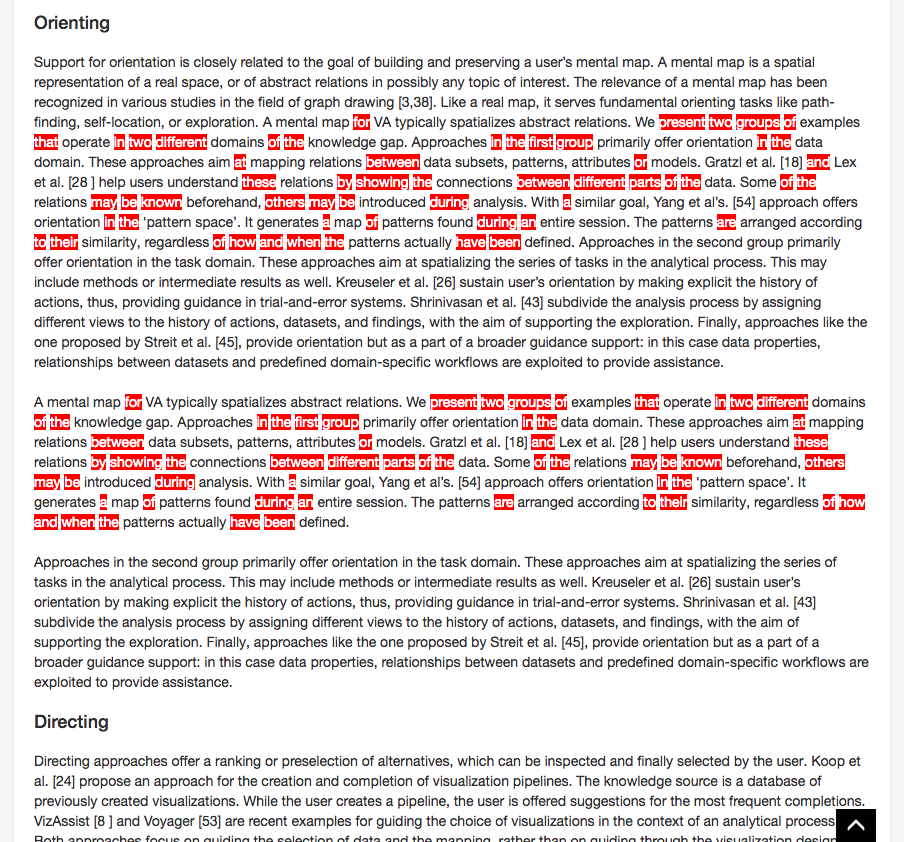
\includegraphics[width=\columnwidth]{textview}
 \caption{Text-Viewer (Markierungen verweisen auf F\"ullw\"orter in dem selektierten Unterkapitel "Orienting")}
 \label{fig:sunburst}
\end{figure}